\documentclass{exam}
%--------------------------------------
%packages
\usepackage[margin=1.35in]{geometry}
\usepackage{amsmath}
\usepackage[shortlabels]{enumitem} %for: being abled to use {enumerate}[a)]
\usepackage{amsthm}%proof environment
\usepackage{color}
\printanswers
\newcommand{\matr}[1]{\mathbf{#1}}
\usepackage{amsfonts}
\usepackage{hyperref}
\usepackage{amssymb}
\usepackage{todonotes}
\usepackage{dsfont}
\usepackage{url}
\usepackage{graphicx}
\usepackage{epstopdf}
\usepackage{algorithm, algpseudocode}
\usepackage{cleveref}
\usepackage[compact,explicit]{titlesec}
\usepackage{caption}
\usepackage[export]{adjustbox}

\newcommand{\lp}{\left(}
\newcommand{\rp}{\right)}
\newcommand{\lb}{\left[}
\newcommand{\rb}{\right]}

\newcommand{\norm}[1]{\|#1\|}
\newcommand{\likelihood}{\mathcal{L}}
\usepackage{cancel}
\newcommand{\bishop}[1]{Bishop #1}
\newcommand{\newword}[1]{{\bf #1}}
\newcommand{\Data}{\mathcal{D}}
\newcommand{\Model}{\mathcal{M}}
\newcommand{\DataTrain}{\mathcal{D}{{\text train}}}
\newcommand{\DataTest}{\mathcal{D}{{\text test}}}
\newcommand{\N}{N}
\newcommand{\Ntrain}{\N_{train}}
\newcommand{\Ntest}{\N_{test}}
\newcommand{\DataSize}{\N}
\newcommand{\DataIndex}{n}
\newcommand{\cind}{t}
\newcommand{\pind}{\star}

\newcommand{\eye}{{\bf I}}

\newcommand{\Dim}{D}
\newcommand{\DimIndex}{d}

\newcommand{\DimOut}{K}
\newcommand{\DimOutIndex}{k}
\newcommand{\Identity}{\mathds{1}}
\newcommand{\wavep}{\widetilde{p}}
\newcommand{\waveq}{\widetilde{q}}
\newcommand{\intphi}{\int_{\phivec}}
\newcommand{\inttheta}{\int_{\thetavec}}
\DeclareMathOperator*{\E}{\mathbb{E}}
\DeclareMathOperator*{\ED}{\mathbb{E}_{\Data}}
\DeclareMathOperator*{\V}{\mathbb{V}}
\DeclareMathOperator*{\LL}{L}
\DeclareMathOperator\erf{erf}
\DeclareMathOperator\trace{tr}
\DeclareMathOperator\median{median}
\DeclareMathOperator*{\argmax}{arg\,max}
\DeclareMathOperator*{\argmin}{arg\,min}
\DeclareMathOperator*{\R}{\mathbb{R}}


\newcommand{\expectation}{\E}
\newcommand{\expectationdata}{\ED}
\newcommand{\variance}{\V}
\let\emptyset\varnothing
\newcommand{\loss}{\LL}
\newcommand{\ascalar}{a}
\newcommand{\bscalar}{b}
\newcommand{\xscalar}{x}
\newcommand{\avec}{{\bf \ascalar}}
\newcommand{\bvec}{{\bf \bscalar}}
\newcommand{\xvec}{{\bf \xscalar}}
\newcommand{\xvectest}{\xvec_{\star}}
\newcommand{\Xmat}{{\bf \MakeUppercase\xscalar}}
\newcommand{\tscalar}{t}
\newcommand{\ttest}{\tscalar_{\star}}
\newcommand{\tvec}{{\bf \tscalar}}
\newcommand{\Tmat}{{\bf \MakeUppercase\tscalar}}
\newcommand{\yscalar}{y}
\newcommand{\yvec}{{\bf \yscalar}}
\newcommand{\Ymat}{{\bf \MakeUppercase\yscalar}}
\newcommand{\wscalar}{w}
\newcommand{\wvec}{{\bf \wscalar}}
\newcommand{\wvecopp}{\wvec^{(-i)}}
\newcommand{\wvecML}{\wvec_{\text{MLE}}}
\newcommand{\wvecMAP}{\wvec_{\text{MAP}}}
\newcommand{\wvecs}{\wvec^{(s)}}
\newcommand{\Wmat}{{\bf \MakeUppercase\wscalar}}
\newcommand{\wbias}{\wscalar_0}
\newcommand{\xn}{\xscalar_{\DataIndex}}
\newcommand{\xvecn}{\xvec_{\DataIndex}}
\newcommand{\tvecn}{\tvec_{\DataIndex}}
\newcommand{\tn}{\tscalar_{\DataIndex}}
\newcommand{\ti}{\tscalar_{i}}
\newcommand{\yvecn}{\yvec_{\DataIndex}}
\newcommand{\yn}{\yscalar_{\DataIndex}}
\newcommand{\yfunc}{\yscalar}
\newcommand{\yfunctest}{\yfunc_{\star}}

\newcommand{\zerovec}{ {\bf 0}}
\newcommand{\pivec}{\boldsymbol{\pi}}
\newcommand{\muvec}{\boldsymbol{\mu}}
\newcommand{\muvecN}{\boldsymbol{\mu}_{\N}}
\newcommand{\munotvec}{\muvec_0}
\newcommand{\mnot}{{\bf m_0}}
\newcommand{\mN}{{\bf m}_{\N}}
\newcommand{\mNplus}{{\bf m}_{\N+1}}
\newcommand{\etavec}{\boldsymbol{\eta}}
\newcommand{\tauvec}{\boldsymbol{\tau}}
\newcommand{\tauinv}{\tau^{-1}}
\newcommand{\thetavec}{\boldsymbol{\theta}}
\newcommand{\thetav}{\thetavec}
\newcommand{\phivec}{\boldsymbol{\phi}}
\newcommand{\Thetamat}{\boldsymbol{\Theta}}
\newcommand{\Gammamat}{\boldsymbol{\Gamma}}
\newcommand{\Gammamatinv}{\Gammamat^{-1}}
\newcommand{\phivectest}{\phivec_{\star}}
\newcommand{\Phimat}{\boldsymbol{\Phi}}
\newcommand{\phivv}{\phivec}
\newcommand{\phivecn}{\phivec_{\DataIndex}}
\newcommand{\phiveci}{\phivec_{i}}
\newcommand{\Sigmamat}{\boldsymbol{\Sigma}}
\newcommand{\SigmamatN}{\Sigmamat_N}
\newcommand{\Sigmamatnot}{\Sigmamat_0}
\newcommand{\Sigmamatinv}{\Sigmamat^{-1}}
\newcommand{\Smat}{{\bf S}}
\newcommand{\SmatN}{\Smat_{\N}}
\newcommand{\Smatnot}{\Smat_0}
\newcommand{\Smatinv}{\Smat^{-1}}
\newcommand{\SmatNplus}{\Smat_{\N+1}}
\newcommand{\SmatNplusinv}{\Smat_{\N+1}^{-1}}
\newcommand{\Betafunc}{\mathcal{B}}
\newcommand{\G}{\mathcal{G}}

\newcommand{\betatest}{\beta_{\star}}
\newcommand{\Amat}{{\bf A}}
\newcommand{\prodnn}{\prod_{n=1}^N}
\newcommand{\prodkk}{\prod_{k=1}^K}
\newcommand{\prodid}{\prod_{i=1}^D}
\newcommand{\proddd}{\prod_{d=1}^D}
\newcommand{\prodiK}{\prod_{i=1}^K}
\newcommand{\sumnn}{\sum_{n=1}^N}
\newcommand{\sumkk}{\sum_{k=1}^K}
\newcommand{\sumw}{\sum_{w}}
\newcommand{\sumww}{\sumw^W}
\newcommand{\sumid}{\sum_{i=1}^D}
\newcommand{\sumiK}{\sum_{i=1}^K}
\newcommand{\znk}{z_{nk}}
\newcommand{\xni}{x_{ni}}
\newcommand{\muki}{\mu_{ki}}
\newcommand{\Bmat}{{\bf B}}
\newcommand{\Cmat}{{\bf C}}
\newcommand{\Dmat}{{\bf D}}
\newcommand{\Emat}{{\bf E}}
\newcommand{\Fmat}{{\bf F}}
\newcommand{\Gmat}{{\bf G}}
\newcommand{\Hmat}{{\bf H}}
\newcommand{\Imat}{{\bf I}}
\newcommand{\Jmat}{{\bf J}}
\newcommand{\Kmat}{{\bf K}}
\newcommand{\Lmat}{{\bf L}}
\newcommand{\Mmat}{{\bf M}}
\newcommand{\Nmat}{{\bf N}}
\newcommand{\Omat}{{\bf O}}
\newcommand{\Pmat}{{\bf P}}
\newcommand{\Qmat}{{\bf Q}}
\newcommand{\Rmat}{{\bf R}}
%\newcommand{\Smat}{{\bf S}}
%\newcommand{\Tmat}{{\bf T}}
\newcommand{\Umat}{{\bf U}}
\newcommand{\Vmat}{{\bf V}}
%\newcommand{\Wmat}{{\bf W}}
%\newcommand{\Xmat}{{\bf X}}
%\newcommand{\Ymat}{{\bf Y}}
\newcommand{\Zmat}{{\bf Z}}

\makeatletter
\newcommand*{\indep}{%
  \mathbin{%
    \mathpalette{\@indep}{}%
  }%
}
\newcommand*{\nindep}{%
  \mathbin{%                   % The final symbol is a binary math operator
    \mathpalette{\@indep}{\not}% \mathpalette helps for the adaptation
                               % of the symbol to the different math styles.
  }%
}
\newcommand*{\@indep}[2]{%
  % #1: math style
  % #2: empty or \not
  \sbox0{$#1\perp\m@th$}%        box 0 contains \perp symbol
  \sbox2{$#1=$}%                 box 2 for the height of =
  \sbox4{$#1\vcenter{}$}%        box 4 for the height of the math axis
  \rlap{\copy0}%                 first \perp
  \dimen@=\dimexpr\ht2-\ht4-.2pt\relax
      % The equals symbol is centered around the math axis.
      % The following equations are used to calculate the
      % right shift of the second \perp:
      % [1] ht(equals) - ht(math_axis) = line_width + 0.5 gap
      % [2] right_shift(second_perp) = line_width + gap
      % The line width is approximated by the default line width of 0.4pt
  \kern\dimen@
  {#2}%
      % {\not} in case of \nindep;
      % the braces convert the relational symbol \not to an ordinary
      % math object without additional horizontal spacing.
  \kern\dimen@
  \copy0 %                       second \perp
} 
\makeatother

\newcommand{\rvec}{{\bf r}}
\newcommand{\betavec}{{\boldsymbol{\beta}}}
\newcommand{\alphavec}{{\boldsymbol{\alpha}}}
\newcommand{\zvec}{{\bf z}}
\newcommand{\zvecn}{{\zvec_n}}
\newcommand{\zvecopp}{{\bf z}^{(-i)}}
\newcommand{\dvec}{{\bf d}}
\newcommand{\lvec}{{\bf l}}
\newcommand{\mvec}{{\bf m}}
\newcommand{\uvec}{{\bf u}}
\newcommand{\vvec}{{\bf v}}

\newcommand{\X}{\mathcal{X}}

\newcommand{\xvecmean}{\bar{\xvec}}
\newcommand{\xvecnest}{\tilde{\xvec}_n}
\newcommand{\xvecestn}{\xvecnest}
\newcommand{\class}{\mathcal{C}}
\newcommand{\gaus}{\mathcal{N}}
\newcommand{\Q}{\mathcal{Q}}
\newcommand{\sigmoid}{\sigma}

\newtheoremstyle{problemstyle}  % <name>
        {1pt}               % <space above>
        {1pt}             % <space below>
        {\normalfont}   % <body font>
        {}              % <indent amount}
        {\bfseries}
        {\normalfont\bfseries:}         % <punctuation after theorem head>
        {.5em}  % <space after theorem head>
        {}  % <theorem head spec (can be left empty, meaning `normal')>
\theoremstyle{problemstyle}{}


\newtheorem{problem}{Problem}
\usepackage{tkz-graph}
\usepackage{tikz}
\usetikzlibrary{bayesnet}
\usepackage{inputenc}
\allowdisplaybreaks

\newcommand{\shrug}[1][]{%
\begin{tikzpicture}[baseline,x=0.8\ht\strutbox,y=0.8\ht\strutbox,line width=0.125ex,#1]
\def\arm{(-2.5,0.95) to (-2,0.95) (-1.9,1) to (-1.5,0) (-1.35,0) to (-0.8,0)};
\draw \arm;
\draw[xscale=-1] \arm;
\def\headpart{(0.6,0) arc[start angle=-40, end angle=40,x radius=0.6,y radius=0.8]};
\draw \headpart;
\draw[xscale=-1] \headpart;
\def\eye{(-0.075,0.15) .. controls (0.02,0) .. (0.075,-0.15)};
\draw[shift={(-0.3,0.8)}] \eye;
\draw[shift={(0,0.85)}] \eye;
% draw mouth
\draw (-0.1,0.2) to [out=15,in=-100] (0.4,0.95); 
\end{tikzpicture}}

\title{Reinforcement Learning - Homework 2} \date{deadline: December 3, 2018}
\author{Andrii Skliar, 11636785\\ Gabriele Bani, 11636758}

\begin{document}
\maketitle 

% \fbox{
%   \parbox{0.8\textwidth}{
%      During the process of solving the homework problems, I have collaborated with the following colleagues: \\\\
%     % LIST ALL THE COLLABORATORS HERE!
%     \begin{tabular}{c c c c}
%         Gabriele Bani & Gabriele Cesa & Davide Belli & Pascal Esser\\
%         Gautier Dagan & & &
%         % more people? put them here:
%         %  &   &   
%   \end{tabular}\\\\
%   \textit{\small NB: credits for the Latex-format go to Iris Verweij, 2nd year MSc AI Student}.
%   }
% }

% \vspace{0.8cm}

%------------------------------
% Problem 1

\begin{problem}[Instructions]
\ \newline
    (empty for correct numeration)
\end{problem}

\begin{problem}[Gradient Descent Methods]
\ \newline
\begin{enumerate}
    \item Why is the Monte Carlo target, $G_t$ , an unbiased estimate of $v_{\pi}(S_t)$?
    \begin{solutionorlines}[2in]
    The fact that $G_t$ is an unbiased estimate of $v_{\pi}(S_t)$ follows directly from the definition of $v_{\pi}(S_t) = \expectation_{\pi}[G_t| S_t=s]$. So, if we take an expectation of the Monte-Carlo target, we get the definition of $v_{\pi}(S_t)$. Therefore, Monte Carlo target, $G_t$, is an unbiased estimate of $v_{\pi}(S_t)$.
    \end{solutionorlines}
    \item Why does using the Dynamic Programming target
    \begin{equation}
        \sum_{a, s',  r} \pi(a|S_t) p(s',r|S_t,a)[r + \gamma \hat{v}(s',\mathbf{w}_t)]
    \end{equation}
    result in a semi-gradient method?
    \begin{solutionorlines}[2in]
    The main reason is that $r$ will depend on $\hat{v}(s',\mathbf{w}_t), s' \in S$, where $S$ is a set of possible states. This implies, that bootstrapping target depends on vector $\mathbf{w}_t$, which is used for approximating state value and might not correspond to the true state value. 
    
    Therefore, if we update our $\mathbf{w}_t$, the target value will also change, which also means that bootstrapping values will be biased unless we reach true value function, which we don't know and therefore can't check if our function has actually converged to the true value function.
    
    As we are updating our function in the direction of the sum of received reward and estimated target and not real target thus including only part of the gradient, this method is called semi-gradient and not full gradient.
    \end{solutionorlines}
    \item Despite not being unbiased, semi-gradient methods that use bootstrapping have certain advantages w.r.t. Monte Carlo approaches. Why, for example, would you prefer bootstrapping in the Mountain Car problem?
    \begin{solutionorlines}[2in]
    The main benefit of semi-gradient methods that use bootstrapping over Monte Carlo approaches is that we don't need to wait for the end of the episode. Semi-gradient methods that use bootstrapping allow us to update our gradient towards more optimal solution at each timestep without waiting for the episode to end. This might result in faster convergence especially in the cases when we might not be able to reach the end of episode at all when using current policy.
    
    If we look at the Mountain Car problem, initially we have bad policy which will make the car oscillate back and forth at the bottom of the hill without actually being able to solve the problem. This is due to that moving forward seems to yield better rewards because we can reach the top of the hill faster, but in reality it is not possible as we don't have enough force to reach the top. Therefore, with Monte Carlo approach, it might take us extensively long to be able to reach top of the hill thus we might not have even a single episode to learn from in a reasonable time. However, with bootstrapping methods and good initialization, we can see that our model will slowly converge to the optimal policy due to that semi-gradient update happens at each timestep.
    \end{solutionorlines}
\end{enumerate}
\end{problem}


\begin{problem}[Basis functions]
\ \newline
\begin{enumerate}
    \item Tabular methods can be seen as a special case of linear function approximation. Show that this is the case and give the corresponding feature vectors.
            \begin{solutionorlines}[2in]
                We can choose to represent states as one-hot vectors. This means that for an environment with $N$ states, we represent each state with an $N$ dimensional feature vector, which is made of all zeros but a one in the position corresponding of the (index of the) represented state. For example, if we have three states, the representation of the second state will be [0, 1, 0].
                We will have then that the general formula for linear function approximators can be written as, for state $s_k$
                
                \begin{align*}
                \hat{v}(s_k, \mathbf{w}) = \mathbf{w}^T \mathbf{x} = \sum_{i=1}^N w_i x_i(s) = w_k
                \end{align*}
            \end{solutionorlines}
    \item You want to design the feature vectors for a state space with $s = [x, y]$. You expect that $x$ and $y$ interact in some unknown way. How would you design a polynomial feature vector for $s$?
            \begin{solutionorlines}[2in]
                First, we assume that the interactions between the two features will be up to order $n$. These interactions can be fully represented by using a polynomial feature vector in the following way (notice that we use the letter $z$ for features as $x$ is already used for the first dimension of the state):
                \begin{align*}
                    z_{ij}(s) =  x^i y^j, & i=0..n, j=0..n
                \end{align*}
                We have defined here for simplicity of notation a matrix $\mathbf{Z}$ of features, which can be converted to the standard row vector representation by using the vectorizization operation $\mathbf{z} = \text{vec}(\mathbf{Z}) $, which stacks vertically all the columns of $\mathbf{Z}$.
                
            \end{solutionorlines}
    \item What happens to the size of the polynomial feature vector if the number of variables in your state space increases?
            \begin{solutionorlines}[2in]
                The size of the polynomial feature vector for a $k$ dimensional state space representation, using polynomials up to order $n$, is $(n+1)^k$. Thus, we can see that if the number of variables $k$ in the state space representation increases, then the number of features needed to represent it using polynomials of up to order $n$ (which is fixed) increases exponentially.
            \end{solutionorlines}
    \item You are working on a problem with a state space consisting of two dimensions. You expect that one of them will have a larger impact on the performance than the other. How might you encode this prior knowledge in your basis function?
            \begin{solutionorlines}[2in]
                Encoding prior knowledge on a problem can be made in different ways, depending on the type of basis functions we are working with. For example, if we are using polynomials, we can use higher order terms for the dimension with more impact on performance. When using RBF instead, we can use different variances for the two dimensions, so that we attribute more importance to one of the two. In tile coding we can instead use different types of tiles than just vertical and horizontal, and favor tiles that can capture salient changes in the larger impact dimension. In general, depending on the type of features, we can either choose to use more features to represent the most relevant dimension, such as in the case of polynomials, or change the importance of the relevant dimension in the features themselves, such as in the case of RBF.
            \end{solutionorlines}
    \item You can view coarse coding as a special case of Radial Basis Functions. Why?
            \begin{solutionorlines}[2in]
                We can see coarse coding as a simplified version of RBFs. First, notice that in both cases we have a circular area of effect around the coordinate of the center of each circle/RBF. In case of RBF, the effect of each RBF is determined as a continuous function of the distance to the current state. Instead, with coarse coding we have a discrete function which takes only the values one or zero. In particular, we can obtain a circle with center $c$ and width $d$ from a RBF of center $c$ and variance $\sigma^2$, by using the function
                
                \begin{align*}
                    f(s) = \begin{cases} 
                    1 &\mbox{if } \exp\big( \frac{|| s - c||^2}{2\sigma^2}\big)  \ge d \\
                    0 & \mbox{if } \exp\big( \frac{|| s - c||^2}{2\sigma^2}\big) < d \end{cases}
                \end{align*}
            \end{solutionorlines}
\end{enumerate}
\end{problem}

\begin{problem}[Geometry of linear value-function approximation]
Consider the MDP given. It consists of two states with one action, that transition into one another with reward $0$. The features for both states are $\phi = 1$ for state $s_0$ and $\phi = 2$ for state $s_1$. We will now predict the value of the states using $v_w = w \cdot \phi$.
\begin{enumerate}
    \item We can write the Bellman error vector as
    \begin{equation}
        \bar{\delta}_w = B^{\pi} v_w - v_w,
    \end{equation}
    where $B^{\pi}$ is the Bellman operator. What is the Bellman error vector after initialization with $w=1$ and using $\gamma=1$?
    \begin{solutionorlines}[2in]
    First, we need to write down the definition of the Bellman operator, which is $(B^{\pi} v_w)(s) = \sum_a \pi(a|s) \sum_{s', r} p(s',r|s,a)[r + \gamma v(s')]$. In our MDP, due to the deterministic policies and transitions, it reduces to $(B^{\pi} v_w)(s) = r + \gamma v(s')$. Now, using this definition and the give way of state value prediction $v_w = w \cdot \phi$, we can calculate Bellman error vector (note, that we define vector of states as $\mathbf{s}=(s_0, s_1)^T$ and $\phi_i$ corresponds to the $\phi$ of state $s_i$):
    \begin{align*}
        v_w(\mathbf{s}) &= \begin{pmatrix}
        w \cdot \phi_0\\
        w \cdot \phi_1
        \end{pmatrix} = \begin{pmatrix}
        1\\
        2
        \end{pmatrix}\\
        (B^{\pi} v_w)(\mathbf{s}) &= \begin{pmatrix}
        r + \gamma (w \cdot \phi_1)\\
        r + \gamma (w \cdot \phi_0)
        \end{pmatrix} = \begin{pmatrix}
        0 + 1 \cdot (1 \cdot 2)\\
        0 + 1 \cdot (1 \cdot 1)
        \end{pmatrix} = \begin{pmatrix}
        2\\
        1
        \end{pmatrix}\\
        \bar{\delta}_w &= \begin{pmatrix}
        (B^{\pi} v_w)(s_0) - v_w(s_0)\\
        (B^{\pi} v_w)(s_1) - v_w(s_1)
        \end{pmatrix} = \begin{pmatrix}
        2 - 1\\
        1 - 2
        \end{pmatrix} = \begin{pmatrix}
        1\\
        -1
        \end{pmatrix}
    \end{align*}
    
    \end{solutionorlines}
    \item What is the Mean Squared Bellman Error?
    \begin{solutionorlines}[2in]
    Assuming that $\mu(s_0) = \mu(s_1) = \frac{1}{2}$, so we are equally interested in accurately estimating value of both states, we can calculate Mean Squared Bellman Error as following:
    \begin{align*}
        \norm{\bar{\delta}_w}_{\mu}^2 = \sum_{s \in \{s_0, s_1\}} \mu(s) v(s)^2 = \frac{1}{2} \cdot 1 + \frac{1}{2} \cdot 1 = 1
    \end{align*}
    \end{solutionorlines}
    \item What $w$ results in the value functions that is closest (in least-squares sense) to the target values $B^{\pi} v_w$?
    \begin{solutionorlines}[2in]
    To calculate $w$ that results in the value functions that is closest (in least-squares sense) to the target values $B^{\pi} v_w$, we simply need to find point on $v_w$ onto which $B^{\pi}v_w$ will be projected. To do that, we should calculate following function: $w = \argmin_{w \in \R}\norm{B^{\pi} v'_w - v_w}^2_{\mu}$ (note that $v'_w$ stands for $v_w$ with current $w=1$).
    \begin{align*}
        f(w) = \norm{\begin{pmatrix}
        2\\
        1
        \end{pmatrix} - \begin{pmatrix}
        1\\
        2
        \end{pmatrix} w
        }_{\mu}^2 &= \norm{
            \begin{pmatrix}
            2 - w\\
            1 - 2w
            \end{pmatrix}
        }_{\mu}^2\\
        &= \frac{1}{2}(2 - w)^2 + \frac{1}{2} (1 - 2w)^2 \\
        &= \frac{1}{2}(4 -4w+w^2 + 1-4w+4w^2)\\
        &= \frac{1}{2}(5w^2-8w+5)\\
        \frac{df}{dw} &= 10w - 8 0\\
        w &= \frac{4}{5}
    \end{align*}
    Therefore, $w=\frac{4}{5}$ results in the value functions that is closest (in least-squares sense) to the target values $B^{\pi} v_w$.
    \end{solutionorlines}
    \item Plot $v_w , B_w^{\pi}$ and $ΠB^{\pi}v_w$. Explain what is happening. (hint: Refer to Figure 11.3 in the book).
    \begin{solutionorlines}[2in]
    As you can see in Figure \ref{fig:plot}, we have value function for defined $w=1$, which is located in a subspace of dimension one in two-dimensional space (i.e. line). This allows us to project it into the larger space with $B_w^{\pi}$ and then project it down onto the line using projection operator. This projection is denoted as $ΠB^{\pi}v_w$. It corresponds to the value $w$, which is the closest to $B_w^{\pi}$ in least-squares sense.\\
    
    So, reaching true value function $v_{\pi}$ consists of sequential interchanging steps of something similar to expectation maximization algorithm, where in expectation step we calculate result of applying Bellman operator $B_w^{\pi}$ with given $w$ and in the maximization step we find $w$ to get as close to $B_w^{\pi}$ using projection operator.
        
    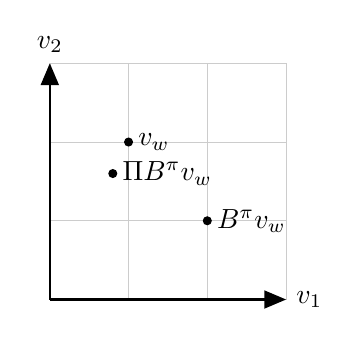
\begin{tikzpicture}
    % help lines
    \draw[step=1,help lines,black!20] (0.0,0.0) grid (3,3);
    % axis
    \draw[thick,->] (0,0) -- (3,0) node[right]{$v_1$};
    \draw[thick,->] (0,0) -- (0,3) node[above]{$v_2$};
    % points
    \foreach \Point/\PointLabel in {(1,2)/v_w, (2,1)/B^{\pi} v_w, (0.8,1.6)/{\Pi B^{\pi}v_w}}
    \draw[fill=black] \Point circle (0.05) node[right] {$\PointLabel$};
    \label{fig:plot}
    \end{tikzpicture}
    
    \end{solutionorlines}
\end{enumerate}
\end{problem}

\begin{problem}[Neural Networks]
\ \newline

\begin{enumerate}
    \item Consider the state distribution, $\mu(s)$. How does it depend on the parameters of the value function approximator?
            \begin{solutionorlines}[2in]
                It depends on the parameters of the value function approximator through the policy $\pi(a| s)$. In fact, changing the parameters of the value functiona approximator also changes the resulting policy, which in turns changes the fraction of time spent in each state, which is represented by $\mu(s)$
            \end{solutionorlines}
    \item How does this differ from standard (un-)supervised learning problems?
            \begin{solutionorlines}[2in]
                This differs from supervised and unsupervised learning asa there the targets and the weightings (when present) are fixed and do not depend on the learnable parameters, while in this case both $\mu_(s)$ and the targets depend by the parametrization. 
                
                Also, in supervised/unsupervised learning the data are fixed and chosen in advance, while in reinforcement learning we dynamically explore the environment, often without fully knowing is dynamics, and the data seen can be different based on our current policy, for example. 
            \end{solutionorlines}
    \item What does this mean for the weighting of the errors (such as in e.g. Eq. 9.1)?
            \begin{solutionorlines}[2in]
                This means that the errors made in each state are weighted differently based on the values of $\mu(s)$. This makes intuitive sense, as when minimizing the mean squared value error, we want errors made in states which are visited more often to be weighted more.
            \end{solutionorlines}
    \item The DQN paper [1] relies, amongst others, on the use of an earlier idea called experience replay [2]. What does this trick do that is important for the algorithm?
            \begin{solutionorlines}[2in]
                Memory replay addresses the problems that neural networks have when trained online. One main drawback of neural networks is that they suffer from \textit{catastrophic forgetting}, which means that they tend to forget information learned in previous samples, the more samples are seen. So, by having a memory and allowing sampling of already seen states, we can partially address the problem as the network can see the same state multiple times. 
                
                Furthermore, typically first order optimizers require the data to be independent in order to converge to good local minima. This is not the case in reinforcement learning, where experience is gained online and thus samples are very related in the same episode. By training only on data sampled on the replay memory, we address the dependence problem as we take random samples from the past.
            \end{solutionorlines}
    \item An other important trick is the use of a separate target network that is frozen for periods of time. What does this trick do that is important for the algorithm?
            \begin{solutionorlines}[2in]
                Using a separate target network is important to stabilize the learning process and prevent drastic changes in the policy. If we would not use a separate target network, then every update to the action-value function would also modify the target of the update, which can lead to oscillations or divergence of the policy. Thus, updating only periodically the target network allows the action-value function to approximate a stable target, and makes oscillations or divergence less likely.
            \end{solutionorlines}
    
\end{enumerate}
\end{problem}

\setcounter{section}{5}
\section{Policy Gradient}

\subsection{Policy Gradient: REINFORCE}
\ \newline
In the lecture, we have seen that introducing a constant baseline b does not introduce a bias to our policy gradient.
\begin{align*}
    \nabla J = \expectation\left[\left(G(\tau) - b\right) \nabla \log p(\tau) \right]
\end{align*}
We now want to consider the variance when introducing a baseline.
\begin{enumerate}
    \item Derive the optimal constant baseline that minimizes the variance of the policy gradient. Interpret your result.
    \begin{solutionorlines}[2in]
    \begin{align*}
        \variance_{\tau}[(G_{\tau} - b) \nabla \log p(\tau)] &= \expectation_{\tau}[(G_{\tau} - b)^2 (\nabla \log p(\tau))^2] - (\expectation_{\tau}[(G_{\tau} - b) \nabla \log p(\tau)])^2\\
        &=  \expectation_{\tau}[(G_{\tau}^2 - 2 b G_{\tau} + b^2) (\nabla \log p(\tau))^2] - (\expectation_{\tau}[(G_{\tau} - b) \nabla \log p(\tau)])^2\\
        &= \expectation_{\tau}[(G_{\tau} (\nabla \log p(\tau)))^2] - 2b \expectation_{\tau}[G_{\tau} (\nabla \log p(\tau))^2] + b^2\expectation_{\tau}[(\nabla \log p(\tau))^2]\\
        &- (\expectation_{\tau}[(G_{\tau} - b) \nabla \log p(\tau)])^2\\
        &= \variance[G_{\tau} (\nabla \log p(\tau))] - 2b \expectation_{\tau}[G_{\tau} (\nabla \log p(\tau))^2] + b^2\expectation_{\tau}[(\nabla \log p(\tau))^2]\\
    \end{align*}
    Now, to minimize variance, we can find extremum point of it, which will also correspond to the minimum point.
    \begin{align*}
        \frac{\partial\variance_{\tau}[(G_{\tau} - b) \nabla \log p(\tau)]}{\partial b} &= -2 \expectation_{\tau}[G_{\tau} (\nabla \log p(\tau))^2] + 2b\expectation_{\tau}[(\nabla \log p(\tau))^2]=0\\
        2b\expectation_{\tau}[(\nabla \log p(\tau))^2] &= 2 \expectation_{\tau}[G_{\tau} (\nabla \log p(\tau))^2]\\
        b &= \frac{\expectation_{\tau}[G_{\tau} (\nabla \log p(\tau))^2]}{\expectation_{\tau}[(\nabla \log p(\tau))^2]}
    \end{align*}
    \end{solutionorlines}
    \item Consider the simple example from the lecture in a bandit setting (i.e. no states):
    \begin{align*}
        r &= a + 2\\
        a &\sim \N(\theta, 1)\\
        \nabla_{\theta} \log \pi(a) &= a - \theta
    \end{align*}
    Can you argue what should be the optimal constant baseline in this case? You can use your result from 1.
    \begin{solutionorlines}[2in]
    \ \newline
    \begin{align*}
        b &= \frac{\expectation_{\tau \sim \pi_{\theta}(\tau)}[G_{\tau} (\nabla_{\theta} \log p(\tau))^2]}{\expectation_{\tau \sim \pi_{\theta}(\tau)}[(\nabla_{\theta} \log p(\tau))^2]}\\
        &= \frac{\expectation_{a}[G_{a} (\nabla \log p(a))^2]}{\expectation_{a}[(\nabla \log p(a))^2]}\\
        &= \frac{\expectation_{a}[(a+2)(a-\theta)^2]}{\expectation_{a}[(a-\theta)^2]}\\
        &= \frac{\expectation_{a}[a^3 - 2\theta a^2 + a \theta^2 + 2a^2 - 4a \theta + 2 \theta^2]}{\expectation_{a}[a^2 -2 a \theta +\theta^2]}\\
        &= \frac{\expectation_{a}[a^3] + 2(1-\theta) \expectation_{a}[a^2] + (\theta^2 -4 \theta)\expectation_{a}[a] + 2\theta^2}{\expectation_{a}[a^2] - 2\theta \expectation_{a}[a] + \theta^2}\\
        &= \frac{\theta^3 + 3\theta + 2(1-\theta)(1+\theta^2) + (\theta^2 -4\theta)\theta + 2\theta^2}{(1 + \theta^2 -2\theta^2 + \theta^2)} \tag{using known moments of Gaussian distribution}\\
        &= \theta^3 + 3\theta + 2 + 2 \theta^2 -2 \theta -2\theta^3 + \theta^3 -4\theta^2 + 2\theta^2\\
        &= \theta + 2
    \end{align*}
    \end{solutionorlines}
    \item Now, consider a baseline that is not constant, but dependent on the state $b(s_t)$. We want to establish that in this case, the policy gradient remains unbiased. Show that
    \begin{align*}
        \expectation_{\tau}[b(s_t) \nabla \log{p(\tau)}] = 0
    \end{align*}
    Hint: you can use the linearity of expectation or the law of iterated expectation to ”decouple” parts of the full trajectory $\tau$.
    \begin{solutionorlines}[2in]
    \ \newline
    \begin{align*}
    \expectation_{\tau}[b(s_t) \nabla \log{p(\tau)}] &= \sum_{t=1}^T \expectation_{\tau}\left[b(s_t) \nabla \log{\pi(a_t|s_t)}\right]\\
    &= \sum_{t=1}^T \expectation_{a_t, s_t}\left[b(s_t) \nabla \log{\pi(a_t|s_t)}\right]\\
    &= \sum_{t=1}^T \expectation_{s_t}\left[\sum_{a_t} \pi(a_t|s_t) b(s_t) \nabla \log{\pi(a_t|s_t)}\right]\\
    &= \sum_{t=1}^T \expectation_{s_t}\left[\sum_{a_t} \pi(a_t|s_t) b(s_t) \frac{\nabla\pi(a_t|s_t)}{\pi(a_t|s_t)} \right]\\
    &= \sum_{t=1}^T \expectation_{s_t}\left[\sum_{a_t} b(s_t) \nabla\pi(a_t|s_t) \right]\\
    &= \sum_{t=1}^T \expectation_{s_t}\left[ b(s_t) \sum_{a_t} \nabla \pi(a_t|s_t) \right]\\
    &= \sum_{t=1}^T \expectation_{s_t}\left[ b(s_t)  \nabla \sum_{a_t} \pi(a_t|s_t) \right]\\
    &= \sum_{t=1}^T \expectation_{s_t}\left[ b(s_t)  \nabla 1 \right]\\
    &= 0 
    \end{align*}
    \end{solutionorlines}
\end{enumerate}


\subsection{Policy Gradient: Compatible Function Approximation Theorem}
\ \newline
Consider the actor-critic method that optimizes the expected return J using the gradient

\begin{align*}
    \nabla J = \expectation_{\tau} \bigg[ \sum_{t=1}^{T} \nabla \log \pi (a_t | s_t) q_{\pi}(s_t, a_t) \bigg]
\end{align*}

where $\pi$ is our parameterized policy (actor) and $q_{\pi}$ is the true state-action value under policy $\pi$. In the lecture we have seen that we can approximate $q_{\pi}$ with a parameterized value function $\hat{q}_w$ which is unbiased if it fulfills the condition
\begin{align*}
    \nabla_w \hat{q}_w &= \nabla_{\theta} \log \pi_{\theta} (s, a) \\
    \text{e.g.} \hat{q}_w &= w^T \nabla_{\theta} \log \pi_{\theta} (s, a)
\end{align*}

\begin{enumerate}
    \item Show that $\expectation_a \big[ \hat{q}_w(s, a) \big] = 0, \forall s \in S$ Briefly interpret this result.
            \begin{solutionorlines}[2in]
                In the case of linear function approximator, we have
                \begin{align*}
                \expectation_a \big[ \hat{q}_w(s, a) \big] &= \expectation_a \big[ w^T \nabla_{\theta} \log \pi_{\theta} (a | s) \big] \\
                &=  w^T \sum_a \pi_{\theta}(a | s) \nabla_{\theta} \log \pi_{\theta} (a | s) \\
                &= w^T \sum_a \pi_{\theta}(a | s) \frac{\nabla_{\theta} \pi_{\theta} (a | s)}{\pi_{\theta} (a | s)} \\
                &= w^T \sum_a \nabla_{\theta} \pi_{\theta} (a | s) \\
                &= w^T \nabla_{\theta} ( \sum_a   \pi_{\theta} (a | s) ) \\
                &= w^T \nabla_{\theta} 1 \\
                &= 0
                \end{align*}
                
                We can see that our estimation $\hat{q}(s, a)$ is not actually an estimator of the true action-value function $q_\pi$, as its espected value is 0 and not $q_\pi$. However, this is reasonable, as we only care about satisfying the compatible function approximation theorem, which guarantees that the average of the gradients using our estimation $\hat{q}(s, a)$ is the same as the average using the true action-value function, so that the actor receives correct gradients.
            \end{solutionorlines}
    \item Evaluate the expectation $\expectation_a \big[ q_{\pi} (s, a) - v_{\pi} (s),  \big], \forall s \in S$. The term $A(s, a) = q_{\pi} (s, a) - v_{\pi} (s) $ is also known as the advantage function.
            \begin{solutionorlines}[2in]
            \begin{align*}
                \expectation_a \big[ q_{\pi} (s, a) - v_{\pi} (s),  \big] &= \expectation_a [q_{\pi} (s, a)] - \expectation_a [v_{\pi} (s)] \\
                    &= v_{\pi} (s) - v_{\pi} (s) \\
                    &= 0
            \end{align*}
            \end{solutionorlines}
    \item What do you conclude from the results in 1 and 2?
            \begin{solutionorlines}[2in]
                We have that the expectation of our approximation $\hat{q}(s, a)$ is the same as the advantage function. Therefore, optimizing $\hat{q}(s, a)$ can be also seen as optimizing the advantage function.
            \end{solutionorlines}
    \item Consider the following policy
    
    \begin{align*}
        \pi_{\theta}(s, a) = \frac{e^{\theta^T \phi_{sa}}}{\sum_b e^{\theta^T \phi_{sb}}}
    \end{align*}
            corresponding to a softmax with linear parametrization with respect to the state-action features $\phi_{sa}$ . Give an expression for the parametrization of $\hat{q}_w$ that satisfies the compatible function approximation theorem.
            \begin{solutionorlines}[2in]
            To satisfy the compatible function approximation theorem, we can use a linear function approximator $\hat{q}_w = w^T \nabla_{\theta} \log \pi_{\theta} (s, a)$.
            We first calculate the derivative with respect to the log policy

            \begin{align*}
                \nt \log \pi_{\theta} (s, a) &= \nt \log \frac{\pa}{\spa} \\
                &= \frac{\spa}{\pa} \nt \frac{\pa}{\spa} \\
                &= \frac{\spa}{\pa} \frac{(\nt \pa) \spa - \pa \nt  \spa}{(\spa)^2} \\
                &= \frac{1}{\pa} \frac{\phi_{sa} \pa \spa - \pa \sum_b \phi_{sb} e^{\theta^T \phi_{sb}} }{\spa} \\
                &=  \frac{\phi_{sa} \spa - \sum_b \phi_{sb} e^{\theta^T \phi_{sb}} }{\spa} \\
                &= \phi_{sa} - \sum_b \phi_{sb} \frac{ e^{\theta^T \phi_{sb}}}{\spa} \\
                &= \phi_{sa} - \sum_b  \pi (s, b)\phi_{sb}
            \end{align*}
            Using this result, we can express $\hat{q}_w$ as
            \begin{align*}
                \hat{q}_w &= w^T \nabla_{\theta} \log \pi_{\theta} (s, a) \\
                &= w^T (\phi_{sa} - \sum_b  \pi (s, b)\phi_{sb}) \\
            \end{align*}
            
            \end{solutionorlines}
    \end{enumerate}


\subsection{Policy Gradient: Natural Gradient}
In this section we parameterize our policy with a univariate Gaussian probability density over real-valued actions. We consider a stateless bandit scenario where you can assume that an episode solely consists of one action and one reward. Mean and variance are learned.
\begin{align*}
    \pi(a | \theta) = \frac{1}{\sigma(\theta_{\sigma}) \sqrt{2\pi}} \exp \bigg( - \frac{(a - \mu(\theta_{\sigma}))^2}{2\sigma(\theta_{\sigma})^2} \bigg)
\end{align*}
where we approximate the mean with a single parameter and the standard deviation with the exponential of a parameter
\begin{align*}
    \mu(\theta_{\mu}) = \theta_{\mu}\\
    \sigma(\theta_{\sigma}) = \exp (\theta_{\sigma})
\end{align*}

\begin{enumerate}
    \item Calculate $\nt \log \pi(a | \theta)$ w.r.t. $\tp$ and $\ts$
        \begin{solutionorlines}[2in]
            \begin{align*}
                \nabla_{\theta_{\mu}} \log \pi(a | \theta) &= \nabla_{\theta_{\mu}} \bigg( - \frac{(a - \theta_{\theta_{\mu}})^2}{2\sigma(\theta_{\sigma})^2} \bigg) - \nabla_{\theta_{\mu}}  \log ( \sigma(\theta_{\sigma}) \sqrt{2\pi} )\\
                &= \nabla_{\theta_{\mu}} \bigg( - \frac{(a - \theta_{\mu})^2}{2\sigma(\theta_{\sigma})^2} \bigg) \\
                &= - \frac{1}{2\sigma(\theta_{\sigma})^2}\nabla_{\theta_{\mu}}(a - \theta_{\mu})^2 \\
                &= - \frac{1}{2\sigma(\theta_{\sigma})^2} 2(a - \theta_{\mu}) (-\theta_{\mu}) \\
                &= \frac{(a - \theta_{\mu})}{\sigma(\theta_{\sigma})^2} \\
                &= \frac{(a - \theta_{\mu})}{\exp(\theta_{\sigma})^2} \\
                &= e^{-2\theta_\sigma}(a - \theta_{\mu})
            \end{align*}
            
            \begin{align*}
                \nabla_{\sigma} \log \pi(a | \theta) &= \nabla_{\sigma} \bigg( - \frac{(a - \theta_{\mu})^2}{2\sigma(\theta_{\sigma})^2} \bigg) - \nabla_{\sigma} \log ( \sigma(\theta_{\sigma}) \sqrt{2\pi} )\\
                &=\nabla_{\sigma} \bigg( - \frac{(a - \theta_{\mu})^2}{2} \frac{1}{\sigma(\theta_{\sigma})^2} \bigg) -  \frac{1}{\sigma(\theta_{\sigma}) \sqrt{2\pi}}  \sqrt{2\pi} \\
                &= \frac{(a - \theta_{\mu})^2}{\sigma(\theta_{\sigma})^3} - \frac{1}{\sigma(\theta_{\sigma}) } \\
                %&= \frac{(a - \theta_{\mu})^2 - \sigma(\theta_{\sigma})^3}{\sigma(\theta_{\sigma})^3}
            \end{align*}
            
            \begin{align*}
                \nabla_{\theta_\sigma} \log \pi(a | \theta) &= \nabla_{\sigma} [\log \pi(a | \theta) ] \nabla_{\theta_{\sigma}} \sigma(\theta_{\sigma}) \\
                &= \bigg( \frac{(a - \theta_{\mu})^2}{\exp(\theta_{\sigma})^3} - \frac{1}{\exp(\theta_{\sigma}) } \bigg)  \exp(\theta_{\sigma}) \\
                &= \frac{(a - \theta_{\mu})^2}{\exp(\theta_{\sigma})^2} - 1\\
                &= e^{-2\theta_\sigma}(a - \theta_{\mu})^2 - 1
            \end{align*}
        \end{solutionorlines}
    \item Why would we want use the natural policy gradient as opposed to the "vanilla" policy gradient?
        \begin{solutionorlines}[2in]
            
            The vanilla policy gradient updates are dependent on the learning rate, and based on the magnitude of the gradients this can lead to worse policies after an update. This does not happen when using natural gradients, which guarantee an improvement in the policy. Also, the natural gradient is independent on the parametrization of the policy, and make the improvements directly in the policy space rather than the parameter space. This is done through the fisher information matrix F, which measures the curvature of the policy with respect to the model parameters. Notice also that the natural gradient constraints the actual amount of change in the policy at each step.
            
            These features make the natural more reliable in terms of quality of updates, and typically lead to better policies.
            
        \end{solutionorlines}
    \item By applying the natural policy gradient we want to the solve the contraint optimization problem
        \begin{align*}
            \theta^{*} - \theta_0 = \max_{d\theta} J(\theta_0 + d\theta) \   \text{s.t.} \   d\theta^T F_{\theta} d\theta = c
        \end{align*}
    where we limit our gradient change to $c$ in KL-divergence between the old and updated policy. The fisher information matrix $F$ and the natural policy gradient update step is then given by
    \begin{align*}
        &F_{\theta} = \expectation_{\tau} \big[ \nabla_{d\theta} \log \pi(a | \theta_0 + d\theta) \nabla_{d\theta} \log \pi(a | \theta_0 + d\theta)^T \big] \\
        &\theta^{*} - \theta_0 \sim F^{-1} \nt J(\theta_0)
    \end{align*}
    Calculate the Fisher information matrix $F_{\theta}$ for our Gaussian policy.
        \begin{solutionorlines}[2in]
            \begin{align*}
                \nabla_{d\theta} \log \pi(a | \theta_0 + d\theta) &= \begin{bmatrix}
                    \nabla_{\theta_\mu} \log \pi(a | \theta) \\
                    \nabla_{\theta_\sigma} \log \pi(a | \theta) \\
                \end{bmatrix} =
                \begin{bmatrix}
                    e^{-2\theta_\sigma}(a - \theta_{\mu}) \\
                    e^{-2\theta_\sigma}(a - \theta_{\mu})^2 - 1 \\
                \end{bmatrix}
            \end{align*}
            
            \begin{align*}
                \nabla_{d\theta} \log \pi(a | \theta_0 + d\theta) &\nabla_{d\theta} \log \pi(a | \theta_0 + d\theta)^T = \begin{bmatrix}
                    \nabla_{\theta_\mu} \log \pi(a | \theta) \\
                    \nabla_{\theta_\sigma} \log \pi(a | \theta) \\
                \end{bmatrix} \big[ \nabla_{\theta_\mu} \log \pi(a | \theta), \nabla_{\theta_\sigma} \log \pi(a | \theta) \big] \\
                &= \begin{bmatrix}
                    e^{-2\theta_\sigma}(a - \theta_{\mu}) \\
                    e^{-2\theta_\sigma}(a - \theta_{\mu})^2 - 1  \\
                \end{bmatrix} \big[ e^{-2\theta_\sigma}(a - \theta_{\mu}), e^{-2\theta_\sigma}(a - \theta_{\mu})^2 - 1 \big] \\
                &= \begin{bmatrix}
                    e^{-4\theta_\sigma}(a - \theta_{\mu})^2  & e^{-4\theta_\sigma}(a - \theta_{\mu})^3 - e^{-2\theta_\sigma}(a - \theta_{\mu}) \\
                    e^{-4\theta_\sigma}(a - \theta_{\mu})^3 - e^{-2\theta_\sigma}(a - \theta_{\mu})   & e^{-4\theta_\sigma}(a - \theta_{\mu})^4 -2 e^{-2\theta_\sigma}(a - \theta_{\mu})^2 +1
                \end{bmatrix}
            \end{align*}
            
            
            Before calculating the expectation of the matrix, we write down the known results for the central moments of the univariate gaussian distribution
            
            \begin{align*}
                \expectation_a [a - \theta_\mu] &=  0 \\
                \expectation_a [(a - \theta_\mu)^2] &= \variance(a) = e^{2\ts}\\
                \expectation_a [(a - \tmu)^3] &= 0 \\
                \expectation_a [(a - \tmu)^4] &= 3 \variance(a)^2 = 3 e^{4\ts}\\
            \end{align*}
            Where $\mu_3$
            Using the same approach as in 6.1.3 where we have shown that expectation of the trajectories can be simplified down to expectation over actions, we get following Fisher Information Matrix:
            
            \begin{align*}
                F_{\theta} &= \begin{bmatrix}
                \expectation_a{\left[e^{-4\theta_\sigma}(a - \theta_{\mu})^2\right]} & \expectation_a{\left[e^{-4\theta_\sigma}(a - \theta_{\mu})^3 - e^{-2\theta_\sigma}(a - \theta_{\mu})\right]} \\
                \expectation_a{\left[e^{-4\theta_\sigma}(a - \theta_{\mu})^3 - e^{-2\theta_\sigma}(a - \theta_{\mu})\right]}   & \expectation_a{\left[e^{-4\theta_\sigma}(a - \theta_{\mu})^4 -2 e^{-2\theta_\sigma}(a - \theta_{\mu})^2\right]} +1
                \end{bmatrix}\\
                &=\begin{bmatrix}
                e^{-4\theta_\sigma} \expectation_a{\left[(a - \theta_{\mu})^2\right]} & e^{-4\theta_\sigma} \expectation_a{\left[(a - \theta_{\mu})^3\right]} - e^{-2\theta_\sigma} \expectation_a{\left[(a - \theta_{\mu})\right]} \\
                e^{-4\theta_\sigma}\expectation_a{\left[(a - \theta_{\mu})^3\right]} - e^{-2\theta_\sigma}\expectation_a{\left[(a - \theta_{\mu})\right]}   & e^{-4\theta_\sigma}\expectation_a{\left[(a - \theta_{\mu})^4\right]} -2 e^{-2\theta_\sigma}\expectation_a{\left[(a - \theta_{\mu})^2\right]} + 1
                \end{bmatrix}\\
                &=\begin{bmatrix}
                e^{-4\theta_\sigma} e^{2\ts} & e^{-4\theta_\sigma} \cdot 0 - e^{-2\theta_\sigma} \cdot 0 \\
                e^{-4\theta_\sigma} \cdot 0 - e^{-2\theta_\sigma} \cdot 0  & e^{-4\theta_\sigma} \cdot 3 e^{4\ts} -2 e^{-2\theta_\sigma}e^{2\ts} +1
                \end{bmatrix}\\
                &=\begin{bmatrix}
                e^{-2\theta_\sigma}  & 0\\
                0  & 3 - 2  + 1
                \end{bmatrix}\\
                &=\begin{bmatrix}
                e^{-2\theta_\sigma}  & 0\\
                0  & 2
                \end{bmatrix}
            \end{align*}
            
        \end{solutionorlines}
    \item Explain the effect of the Fisher information matrix on gradient updates of $\theta_{\mu}$ when using the natural gradient.
        \begin{solutionorlines}[2in]
            To do gradient update with Fisher information matrix, we need to multiply gradient by the inverse of Fisher information matrix. As our information matrix is diagonal, we can see that taking an inverse of it is the same as taking an inverse of each element on the diagonal. Also, in that case we can treat elements on the diagonal of Fisher information matrix as scaling factors for corresponding parameters.\\
            
            Therefore, when we multiply $\theta_{\mu}$ by $e^{2\theta_\sigma}$, it increases the update, which means that this direction is less sensitive to the updates. Fish information matrix thus controls which directions of the gradient should be updated more in order to reach optimal policy and which should be updated less. This also reminds of adaptive learning rate approach used in deep learning.  
        \end{solutionorlines}
    \item Consider a slightly different parametrization of the standard deviation as 
    \begin{align*}
        \sigma(\ts) = \ts
    \end{align*}
    where we simply learn σ directly. We will ignore that the variance can technically become negative in this case. Calculate $\nabla  \log \pi (a | \theta)$ and $F$ θ w.r.t. $\ts$ for this alternative parametrization.
        \begin{solutionorlines}[2in]
            Using the result found in the first part of this exercise, we have  
            \begin{align*}
                \nabla_{\sigma} \log \pi(a | \theta) &= \frac{(a - \theta_{\mu})^2}{\sigma(\theta_{\sigma})^3} - \frac{1}{\sigma(\theta_{\sigma}) } \\
            \end{align*}
            \begin{align*}
                \nabla_{\theta_\sigma} \log \pi(a | \theta) &= \nabla_{\sigma} [\log \pi(a | \theta) ] \nabla_{\theta_{\sigma}} \sigma(\theta_{\sigma}) \\
                &= \bigg( \frac{(a - \theta_{\mu})^2}{\theta_{\sigma}^3} - \frac{1}{\theta_{\sigma} } \bigg)  1 \\
                &= \frac{(a - \theta_{\mu})^2}{\theta_{\sigma}^3} - \frac{1}{\theta_{\sigma}} \\
            \end{align*}
            While for $\tmu$ the result is, reusing the calculations of previous points
            \begin{align*}
                \nabla_{\theta_{\mu}} \log \pi(a | \theta) =  \frac{(a - \theta_{\mu})}{\sigma(\theta_{\sigma})^2} = \frac{(a - \theta_{\mu})}{\theta_{\sigma}^2} \\
            \end{align*}
            
            The Fisher information matrix can be written then as
            \begin{align*}
                \nabla_{d\theta} \log \pi(a | \theta_0 + d\theta) \nabla_{d\theta} \log \pi(a | \theta_0 + d\theta)^T &= \begin{bmatrix}
                    \nabla_{\theta_\mu} \log \pi(a | \theta) \\
                    \nabla_{\theta_\sigma} \log \pi(a | \theta) \\
                \end{bmatrix} \big[ \nabla_{\theta_\mu} \log \pi(a | \theta), \nabla_{\theta_\sigma} \log \pi(a | \theta) \big] \\
                &= \begin{bmatrix}
                    \frac{(a - \theta_{\mu})}{\theta_{\sigma}^2} \\
                    \frac{(a - \theta_{\mu})^2}{\theta_{\sigma}^3} - \frac{1}{\theta_{\sigma}}
                \end{bmatrix}
                \big[ \frac{(a - \theta_{\mu})}{\theta_{\sigma}^2}, \frac{(a - \theta_{\mu})^2}{\theta_{\sigma}^3} - \frac{1}{\theta_{\sigma}}  \big] \\
                &= \begin{bmatrix}
                    \frac{(a - \theta_{\mu})^2}{\theta_{\sigma}^4} & 
                    \frac{(a - \theta_{\mu})^3}{\theta_{\sigma}^5} - \frac{(a - \theta_{\mu})}{\theta_{\sigma}^4}\\
                    \frac{(a - \theta_{\mu})^3}{\theta_{\sigma}^5} - \frac{(a - \theta_{\mu})}{\theta_{\sigma}^4} & \frac{(a - \theta_{\mu})^4}{\theta_{\sigma}^6} - 2\frac{(a - \theta_{\mu})^2}{\theta_{\sigma}^4}  + \frac{1}{\theta_{\sigma}^2}
                \end{bmatrix}
            \end{align*}
            
            As in 6.3.3, we can write
            
            \begin{align*}
                F_\theta &= \begin{bmatrix}
                    \expectation_a [ \frac{(a - \theta_{\mu})^2}{\theta_{\sigma}^4} ] 
                    & \expectation_a [\frac{(a - \theta_{\mu})^3}{\theta_{\sigma}^5} - \frac{(a - \theta_{\mu})}{\theta_{\sigma}^4}]\\
                    \expectation_a [ \frac{(a - \theta_{\mu})^3}{\theta_{\sigma}^5} - \frac{(a - \theta_{\mu})}{\theta_{\sigma}^4}] 
                    & \expectation_a [\frac{(a - \theta_{\mu})^4}{\theta_{\sigma}^6} - 2\frac{(a - \theta_{\mu})^2}{\theta_{\sigma}^4}  + \frac{1}{\theta_{\sigma}^2}]
                \end{bmatrix} \\
                &= \begin{bmatrix}
                    \frac{1}{\ts^2}
                    & 0\\
                    0 
                    & \frac{3\theta_{\sigma}^4}{\theta_{\sigma}^6} - 2 \frac{\theta_{\sigma}^2}{\theta_{\sigma}^4} + \frac{1}{\theta_{\sigma}^2}
                \end{bmatrix} \\
                &= \begin{bmatrix}
                    \frac{1}{\ts^2}
                    & 0\\
                    0 
                    & \frac{3 - 2 + 1}{\theta_{\sigma}^2}
                \end{bmatrix} \\
                &= \begin{bmatrix}
                    \frac{1}{\ts^2}
                    & 0\\
                    0 
                    & \frac{2}{\theta_{\sigma}^2}
                \end{bmatrix}
            \end{align*}
            
        \end{solutionorlines}
    \item Compare how the Fisher information matrix influences the gradient of $\ts$ considering both parametrizations of $\sigma$. Explain your observations.
        \begin{solutionorlines}[2in]
                We can easily see that in the first parametrization, standard deviation will be updated less as $2 < 8$. This is due to the fact that in case of parametrization with exponent, changing $\theta_{\sigma}$ influences the value of $\sigma$ more than in case of linear parametrization. Therefore, Fisher information matrix controls our updates not to change the value of the parameter too radically, which might potentially result in non-converging performance.
        \end{solutionorlines}
        
    \item Suppose our current parameters are $\mu = 0$ and $\sigma = 4$. We now observe an episode with $a = 8$ and $F(\tau) = 1$. Perform a gradient update on $\ts$ with learning rate $\alpha = 0.01$ using the vanilla policy gradient as well as using the natural policy gradient for both parametrizations, i.e. a total of four independent updates. Report the updated values of $\sigma$ and discuss your observations.
        \begin{solutionorlines}[2in]
        The main thing to notice is that in our case with one episode and parametrization on $\boldsymbol{\theta}$, gradient can be calculated as $\nabla_{\boldsymbol{\theta}} J= G(t) \nabla \log \pi(a_t|\boldsymbol{\theta})$.
        
        For the first suggested parametrization, $\sigma = 4, \mu = 0$, therefore $\theta_{\sigma} = \ln 4, \theta_{\mu} = 0$:
            \begin{align*}
                \nabla_{\boldsymbol{\theta}} J &= 1 \cdot \begin{bmatrix}
                e^{-2\theta_\sigma}(a - \theta_{\mu})\\
                e^{-2\theta_\sigma}(a - \theta_{\mu})^2 - 1
                \end{bmatrix}\\
                &= 1 \cdot \begin{bmatrix}
                4^{-2} (8 - 0)\\
                4^{-2} (8 - 0)^2 - 1
                \end{bmatrix}\\
                &= \begin{bmatrix}
                \frac{1}{2} \\
                3
                \end{bmatrix}\\
                \boldsymbol{\theta} &= \boldsymbol{\theta}  + \alpha  \nabla_{\boldsymbol{\theta}} J \tag{Vanilla policy gradient}\\ &= \begin{bmatrix}
                0\\
                \ln 4
                \end{bmatrix} + 0.01 \cdot  \begin{bmatrix}
                \frac{1}{2}\\
                3
                \end{bmatrix} \\
                &\approx \begin{bmatrix}
                0.005\\
                1.416294
                \end{bmatrix}\\
                \mu &= 0.005\\
                \sigma &= 4.121816\\
                \boldsymbol{\theta} &= \boldsymbol{\theta}  + \alpha F_{\boldsymbol{\theta}}^{-1}  \nabla_{\boldsymbol{\theta}} J \tag{Natural policy gradient}\\ 
                &= \begin{bmatrix}
                0\\
                \ln 4
                \end{bmatrix} + 0.01 \cdot 
                \begin{bmatrix}
                e^{-2\theta_\sigma}  & 0\\
                0  & 2
                \end{bmatrix}^{-1} \cdot
                \begin{bmatrix}
                \frac{1}{2}\\
                3
                \end{bmatrix} \\
                &= \begin{bmatrix}
                0\\
                \ln 4
                \end{bmatrix} + 0.01 \cdot 
                \begin{bmatrix}
                \frac{1}{16}  & 0\\
                0  & 2
                \end{bmatrix}^{-1} \cdot
                \begin{bmatrix}
                \frac{1}{2}\\
                3
                \end{bmatrix} \\
                &= \begin{bmatrix}
                0\\
                \ln 4
                \end{bmatrix} + 0.01 \cdot 
                \begin{bmatrix}
                16  & 0\\
                0  & \frac{1}{2}
                \end{bmatrix} \cdot
                \begin{bmatrix}
                \frac{1}{2}\\
                3
                \end{bmatrix} \tag{property of diagonal matrix}\\
                &\approx \begin{bmatrix}
                0\\
                \ln 4
                \end{bmatrix} + 0.01 \cdot 
                \begin{bmatrix}
                8\\
                1.5
                \end{bmatrix}\\
                &\approx \begin{bmatrix}
                0.08\\
                1.401294
                \end{bmatrix}\\
                \mu &= 0.08\\
                \sigma &= 4.060450
            \end{align*}
            
        For the second suggested parametrization, $\sigma = 4, \mu = 0$, therefore $\theta_{\sigma} = 4, \theta_{\mu} = 0$:
            \begin{align*}
                \nabla_{\boldsymbol{\theta}} J &= 1 \cdot \begin{bmatrix}
                 \frac{(a - \theta_{\mu})}{\theta_{\sigma}^2}\\
                \frac{(a - \theta_{\mu})^2}{\theta_{\sigma}^3} - \frac{1}{\theta_{\sigma}}
                \end{bmatrix}\\
                &= 1 \cdot \begin{bmatrix}
                \frac{8}{16}\\
                \frac{64}{62} - \frac{1}{4}
                \end{bmatrix}\\
                &= \begin{bmatrix}
                \frac{1}{2} \\
                \frac{3}{4}
                \end{bmatrix}\\
                \boldsymbol{\theta} &= \boldsymbol{\theta}  + \alpha  \nabla_{\boldsymbol{\theta}} J \tag{Vanilla policy gradient}\\ &= \begin{bmatrix}
                0\\
                4
                \end{bmatrix} + 0.01 \cdot  \begin{bmatrix}
                \frac{1}{2} \\
                \frac{3}{4}
                \end{bmatrix} \\
                &\approx \begin{bmatrix}
                0.005\\
                4.0075
                \end{bmatrix}\\
                \mu &= 0.005\\
                \sigma &= 4.0075\\
                \boldsymbol{\theta} &= \boldsymbol{\theta}  + \alpha F_{\boldsymbol{\theta}}^{-1}  \nabla_{\boldsymbol{\theta}} J \tag{Natural policy gradient}\\ 
                &= \begin{bmatrix}
                0\\
                 4
                \end{bmatrix} + 0.01 \cdot 
               \begin{bmatrix}
                    \frac{1}{\ts^2}
                    & 0\\
                    0 
                    & \frac{2}{\theta_{\sigma}^2}
                \end{bmatrix}^{-1} \cdot
                \begin{bmatrix}
                \frac{1}{2} \\
                \frac{3}{4}
                \end{bmatrix} \\
                &= \begin{bmatrix}
                0\\
                 4
                \end{bmatrix} + 0.01 \cdot 
                \begin{bmatrix}
                \frac{1}{16}  & 0\\
                0  & \frac{2}{16}
                \end{bmatrix}^{-1} \cdot
                \begin{bmatrix}
                \frac{1}{2} \\
                \frac{3}{4}
                \end{bmatrix}\\
                &= \begin{bmatrix}
                0\\
                4
                \end{bmatrix} + 0.01 \cdot 
                \begin{bmatrix}
                16  & 0\\
                0  & 8
                \end{bmatrix} \cdot
                \begin{bmatrix}
                \frac{1}{2} \\
                \frac{3}{4}
                \end{bmatrix} \tag{property of diagonal matrix}\\
                &= \begin{bmatrix}
                0\\
                4
                \end{bmatrix} + 0.01 \cdot 
                \begin{bmatrix}
                8\\
                6
                \end{bmatrix}\\
                &\approx \begin{bmatrix}
                0.08\\
                4.06
                \end{bmatrix}\\
                \mu &= 0.08\\
                \sigma &= 4.06
            \end{align*}
        The observed result in the case of natural gradient confirms our suggestion in 6.6, as, indeed, in the first parametrization we update $\theta_\sigma$ by $0.015$ and in the second parametrization we update it by $0.06$. This is due to the fact that changing parameter of the exponent changes the value of the function much more than when updating parameter of linear function. Therefore, Fisher information matrix keeps our updates more careful.
        
        On the other hand, in the case of vanilla gradient, our update increases for the exponential case, which also means that the value of $\sigma$ changes more rapidly. This might result in that in the case of exponential parametrization, we might never be able to reach the optimal value as we are changing parameter too fast, which is not as bad in the linear case. Natural gradient helps us to avoid this issue. 
        
        Both of these observations can also be seen from the fact that for both parametrizations, value of the $\sigma$ stays very similar when using natural gradient but gets quite different with vanilla gradient.
         \end{solutionorlines}
\end{enumerate}


\bibliographystyle{plain}
\bibliography{bibliography}
\end{document}